% Este arquivo .tex será incluído no arquivo .tex principal. Não é preciso
% declarar nenhum cabeçalho

% Números de telefone comentados nessa seção não foram confirmados, mas ainda
% podem estar funcionando. TODO: conferir devidamente na edição 2015-2016.
\section{Outras necessidades}
\subsection{Supermercados}

No centro de Barão há três supermercados: o Pague Menos (antigo Super Barão ou
``Super Ladrão'') o Pão de Açúcar e o Dalben. Ambos Pague Menos e Pão de Açúcar
são muito caros, mas o Pague Menos tem boas promoções de segunda e terça-feiras.
Cada um é melhor ou mais barato para alguma coisa. Só indo bastante em cada um é
que você pega o jeito.

\begin{figure}[h!]
    \centering
    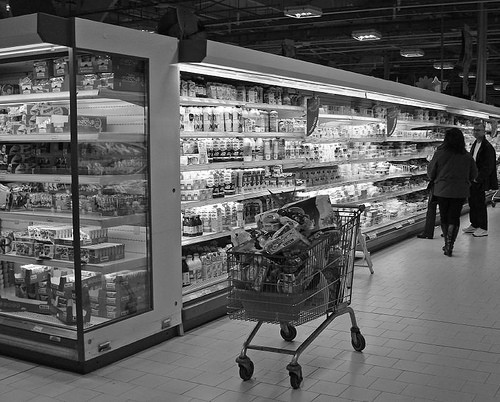
\includegraphics[width=.45\textwidth]{img/barao/supermercado.jpg}
\end{figure}

O Dalben é maior e geralmente tem coisas mais baratas que o Pão de Açúcar. Às
segundas e terças (no Dalben e no Pague Menos) e às terças (no Pão de Açúcar) há
preço promocional de frutas e verduras. O Dalben localiza-se no alto da Avenida
1, na entrada de Barão Geraldo. O Pague Menos funciona de segunda a sábado das
7h às 22h e aos domingos das 8h às 20h, e o Pão de Açúcar funciona de domingo a
quinta-feira das 7h às 23h, às sextas e aos sábados das 7h às 24h. Logo na
frente da moradia, bem na frente do ponto do circular (algo consideravelmente
prático) fica um Dia, que costuma ser um mercado bem barato, além disso, perto
da moradia também tem o Benatti.

Há também lojas de conveniência em diversos postos que embora mais caras que os
supermercados, podem funcionar em horários alternativos ou serem mais perto de
onde você mora.

Em frente ao Terminal Barão há o Recanto Bela Fruta, que não é exatamente um
supermercado, mas é o melhor lugar de Barão para comprar frutas, verduras e
legumes. Vende também algumas coisas de supermercado como pão, leite, iogurte,
Mupy etc. Na estrada da Rhodia, depois da Padaria Di Capri, há a frutaria Rio
das Pedras, que tem preços no nível do Pão de Açúcar e do Pague Menos, mas é
mais próximo pra quem vive na Cidade Universitária 2, por exemplo.

Se você tiver carro, ou conhecer alguém que tenha, junte um pessoal e faça suas
compras no Tenda Atacado ou no Atacadão. Os dois são muito mais baratos que
qualquer supermercado e têm muita variedade. Ah, e nem tudo é atacado, vende
umas coisas a varejo lá também. Para chegar aos dois, saindo de Barão pelo
Tapetão, pegue a D. Pedro sentido Anhanguera. Assim que você entrar na D. Pedro,
você já vai enxergar o Atacadão, à direita. Para ir ao Tenda siga mais um pouco
na D.  Pedro e saia logo depois do CEASA à direita.

Outras opções para quem tem carro são: O Carrefour, localizado na Rodovia D.
Pedro, o Wal-Mart, que fica no Shopping Parque D. Pedro e, andando mais um 
pouquinho na Rodovia D. Pedro, tem o Extra D. Pedro.

\subsection{Utilidades em geral}

\begin{itemize}
    \item  \textbf{Ki-Água}
        \\Telefone: (19) 3289-4659
        \\Endereço: Estrada do Rhodia, 3100

    \item  \textbf{Circuito das Águas}
        \\Telefone: (19) 3289-4930
        \\Endereço: Rua Júlia Leite de Barros, 182

    \item  \textbf{Água Mineral Serrana}
        \\Telefone: (19) 3289-4602
        \\Endereço: Av. Albino J. B. de Oliveira, 658

    \item  \textbf{Real Gás}
        \\Telefone: (19) 3289-1786
        \\Endereço: Rua Eduardo Pereira de Almeida, 570

    \item  \textbf{Genebra Gás}
        \\Telefone: (19) 3289-3622
        \\Endereço: Av. Santa Isabel, 622

    \item  \textbf{Drogaria Vitória}
        \\Telefone: (19) 3289-9926
        \\Endereço: Av. Ruberley Bueretto da Silva, 1015
    
    \item  \textbf{Drogasil}
        \\Telefone: (19) 3249-1449
        \\Endereço: Av. Albino J. B. de Oliveira, 448
        
    % \item  \textbf{Drogaria Nova Barão}
    %     \\Telefone: (19) 3289-6191

    % \item  \textbf{Rede Farmaxima}
    %     \\Telefone: (19) 3289-2824 / (19) 3289-4054
    %     \\Endereço: Av. Dr. Romeu Tortima, 255

    \item  \textbf{New Laundry Lavanderia}
        \\Telefone: (19) 3289-3922
        \\Endereço: Rua Francisca Resende Merciai, 54

    \item  \textbf{Desentupimento 24 horas}
        \\Telefone: (19) 3242-1249

    \item  \textbf{Carpintaria São Jorge de Barão}
        \\Telefone: (19) 3289-3399
        \\Endereço: Av. Santa Isabel, 1882

    \item  \textbf{CPFL (companhia de luz)}
        \\Telefone: 0800-010-1010

    \item  \textbf{Sanasa (companhia de água)}
        \\Telefone: 0800-772-1195

    %\item  \textbf{Luigi Cabelereiro}
    %    \\Telefone: (19) 3288-0198

    \item  \textbf{João Cabelereiros}
        \\Telefone: (19) 3289-3084
        \\Endereço: Rua Orácio Leonardi, 92

    \item  \textbf{Correios -- Centro de Barão}
        \\Endereço: Av. Santa Isabel, 218 -- Centro de Barão
        \\Telefone: (19) 3288-0244

    \item  \textbf{Correios -- Unicamp}
        \\Endereço: Rua Carlos Gomes, 241 -- Campus da Unicamp (próximo ao ginásio e Instituto de Artes)
        \\Telefone: (19) 3289-7288 / (19) 3521-7642
\end{itemize}

\subsection{Bancos}

Bixo, agora que você está na universidade, chegou a hora de tomar vergonha na
cara e abrir uma conta no banco. A menos que você more em Campinas ou muito
perto, essa será a forma principal do papai te mandar dinheiro.

Todos os bancos oferecem algum tipo de conta universitária, que tem tarifas
reduzidas. Os documentos exigidos para abertura de conta costumam ser
identidade, CPF, comprovante de residência (conta de água, luz, telefone, gás --
pode ser do endereço da sua cidade e no nome dos seus pais) e e comprovante de
renda (pode ser no nome dos seus pais).

Além da conta universitária, alguns bancos oferecem uma modalidade de conta
inteiramente sem custo, mas que pode ser operada apenas por meios eletrônicos,
como internet banking, caixa eletrônico, cartão de débito e crédito e telefone.
Enquadram-se nesta categoria as contas eletrônicas do Banco do Brasil e do
Santander e a iConta do Itaú.

Há várias agências bancárias dentro da Unicamp e em Barão Geraldo. Confira onde
se localizam:

\begin{itemize}
    \item  \textbf{Banco do Brasil:} Há três agências: uma localizada perto da
        Reitoria, outra no centro de Barão, perto do Santander, e outra no
        centro de Barão perto do Pague Menos. Há ainda uma agência exclusiva
        para clientes Estilo próxima aos Correios da Unicamp.

    \item  \textbf{Bradesco:} Agência no centro de Barão, do lado do Banco do
        Brasil e em frente do Santander. Próxima ao Terminal Barão.

    \item  \textbf{Caixa Econômica Federal:} Localizada na fren\-te do Pão de
        Açúcar.

    \item  \textbf{Citibank:} Localizado no alto da avenida 2, próximo ao posto
        Shell.

    \item  \textbf{Itaú:} Possui uma agência na Unicamp, próximo à Reitoria e à
        agência do Santander, e outra na avenida Santa Isabel, do lado da
        sorveteria. Existe também o Itaú Personnalité, próximo ao Pão de Açuar e
        ao McDonalds.

    \item  \textbf{Santander:} Há quatro agêncais em Barão: duas localizadas ao
        lado da Reitoria, outra na praça do Ciclo Básico e a outra próxima ao
        Terminal Barão.
\end{itemize}

\subsection{Sebos e livrarias}

Em Barão há três sebos: O Curupira, o Cronópio e o Galpão. Geralmente você não
encontra muita coisa boa de computação neles, mas não custa procurar. O Curupira
fica na rua do Terminal, bem em frente a ele. Não é difícil achar. O Galpão fica
perto do Terminal. Saindo do terminal pela avenida marginal à Albino de
Oliveira, vire a primeira à esquerda e a segunda à direita. Funciona de segunda
à sexta até às 18h. O Cronópio fica na mesma rua do Galpão, só que bem longe,
próximo à padaria Fiori. Seguindo a Santa Isabel, vindo do Centro de Barão, vire
à esquerda na esquina que tem uma pizzaria (antes da Fiori). Vire na primeira à
esquerda e você está no Cronópio (Lá também é um restaurante barato e gostoso).

Na Unicamp há a livraria Toledo, que fica na Faculdade de Educação (Pedago), tem
pouca coisa de Computação lá, mas sempre tem alguma coisa de Matemática. Também
há a livraria da Unicamp (no IEL), tem preços bons mas não tem quase nada de
Exatas. Já a Livraria da Química tem livros de exatas, e geralmente eles
conseguem importar a um preço bom. Outras livrarias são a Fnac (no Shopping D.
Pedro), a Saraiva e a Cultura (no Shopping Iguatemi) e a Siciliano (no Shopping
Galeria).

Mais uma dica: Antes de comprar um livro, veja se você vai usar muito ele, se
não tem bastante na biblioteca, se algum veterano legal não pode te emprestar ou
te vender, ou se não rola tirar xerox. Você compra livro só se você precisar
e/ou quiser muito. Caso vá comprar, atente para livrarias virtuais, que podem
ter preços muito menores (pesquise sempre no Buscapé (\url{buscape.com.br})) e
emitem boletos para você pagar no banco.  Em alguns casos, a livraria da Editora
(localizada no piso térreo da BC) pode trazê-lo por um preço menor ainda --
consulte sempre!

Uma última dica: Não compre o livro de G.A. (MA141). Estude pelo Stewart II
(livro de Cálculo II), pelo Steinbruch ou pelo livro do Paulo Boulos. Os três
são muito melhores que ele. Se você quiser os exercícios para estudar para os
testes pegue na internet ou tire xerox. Use os outros livros para estudar.

\begin{figure}[h!]
    \centering
    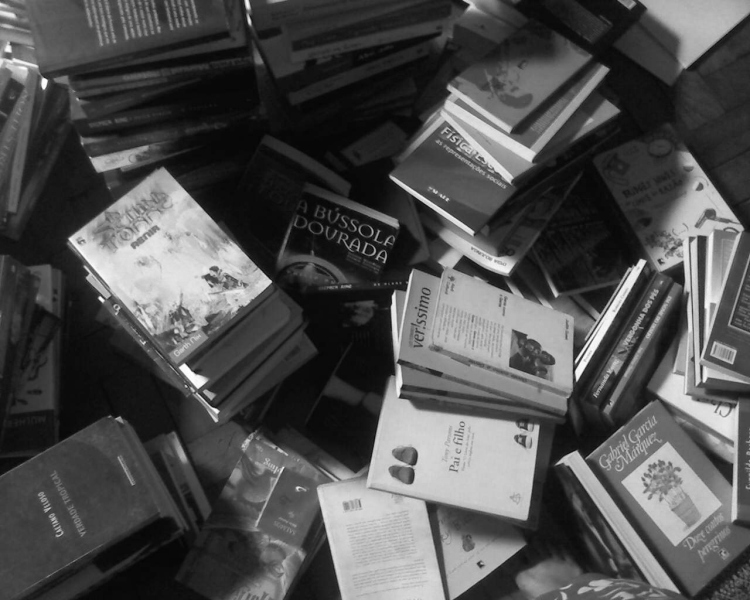
\includegraphics[width=.45\textwidth]{img/barao/sebo.jpg}
\end{figure}

\begin{itemize}
    \item   \textbf{Sebo Galpão}
        \\Endereço: Rua Alberto de Salvo, 201
        \\Telefone: (19) 3289-2044

    \item   \textbf{Sebo Valise de Cronópio}
        \\Endereço: Rua Francisco de Barros Filho, 426
        \\Telefone: (19) 3289-0028
\end{itemize}

\subsection{Bicicletarias}

\begin{itemize}
    \item   \textbf{Rei do Pedal}
        \\Endereço: Av. Santa Isabel, 74
        \\Telefone: (19) 3289-9258

    \item   \textbf{Via Bike}
        \\Endereço: Av. Albino J. B. de Oliveira, 1074
        \\Telefone: (19) 3289-9888
\end{itemize}

\subsection{Escolas de idiomas}

\begin{itemize}
    \item   \textbf{CCAA}
        \\Endereço: Rua Professor Atilio Martini, 421
        \\Telefone: (19) 3249-0202
        \\E-mail: \email{barao@ccaa.com.br}
        \\Site: \url{ccaa.com.br/barao}

    \item   \textbf{CCBEUC -- Centro Cultural Brasil Estados Unidos -- Campinas}
        \\Endereço: Av. Dr. Romeu Tortima, 531
        \\Telefone: (19) 3249-0275
        \\E-mail: \email{admbg@ccbeuc.com.br}
        \\Site: \url{ccbeuc.com.br}
        
    \item   \textbf{Cultura Inglesa}
        \\Endereço: Av. Dr. Romeu Tortima, 538
        \\Telefone: (19) 3249-0275
        \\Site: \url{www.culturainglesasp.com.br}

    \item   \textbf{CNA}
        \\Endereço: Av. Dr. Romeu Tortima, 553
        \\Telefone: (19) 3289-4700
        \\Fax: (19) 3289-4700
        \\E-mail: \email{baraogeraldo@cna.com.br}
        \\Site: \url{cna.com.br/baraogeraldo}

    \item   \textbf{HAVAD}
        \\Endereço: Av. Dr. Romeu Tortima, 522
        \\Telefone: (19) 3288-0012
        \\Fax: (19) 3249-0488
        \\E-mail: \email{havad@havad.com.br}
        \\Site: \url{havad.com.br}

    \item   \textbf{In Touch}
        \\Endereço: Rua Antônio Augusto de Almeida, 517 -- Cidade Universitária
        \\Telefone: (19) 3289-3481
        \\E-mail: \email{secretaria@intouch.art.br}
        \\Site: \url{www.intouch.art.br}

    \item   \textbf{INOVA -- Escola de Inglês}
        \\Endereço: Av. Dr. Romeu Tortima, 391
        \\Telefone: (19) 3288-0071
        \\E-mail: \email{fale@inovalinguas.com.br}
        \\Site: \url{inovalinguas.com.br}

    \item   \textbf{Skill Idiomas}
        \\Endereço: Rua Agostinho Páttaro, 47 (esquina com a do praça do coco)
        \\Telefone: (19) 3289-6240

    \item   \textbf{Wizard}
        \\Endereço: Rua João Batista Antonioli, 90
        \\Telefone: (19) 3289-6199
        \\Site: \url{wizard.com.br}

    \item   \textbf{Yazigi}
        \\Endereço: Av. Dr. Romeu Tortima, 500
        \\Telefone: (19) 3249-2375
        \\Site: \url{yazigi.com.br}
\end{itemize}

\subsection{Igrejas}

\begin{itemize}
    \item   \textbf{IBCU -- Igreja Batista da Cidade Universitária}
        \\Endereço: Rua Tenente Alberto Mendes Jr., 5
        \\Telefone: (19) 3289-4501
        \\E-mail: \email{jovens@ibcu.org.br}
        \\Site: \url{ibcu.org.br}

    \item   \textbf{IBBG -- Igreja Batista de Barão Geraldo}
        \\Endereço: Rua Luiz Vicentim, 284
        \\Telefone: (19) 3289-1793

    \item   \textbf{IPBG -- Igreja Presbiteriana de Barão Geraldo}
        \\Endereço: Rua Francisco Andreo Aledo, 141 (próximo à praça do coco e moradia)
        \\Telefone: (19) 3289-3239

    % \item   \textbf{Igreja do Nazareno Betânia}
    %     \\Endereço: Rua Manoel Antunes Novo, 98
    %     \\Telefone: (19) 3289-7379

    % \item   \textbf{Assembleia de Deus -- Ministério de Belém}
    %     \\Endereço: Rua Júlia Leite de Barros, 54 (próximo à moradia da Unicamp)
    %     \\Telefone: (19) 3249-0035
    %     \\Site: \url{adbarao.com.br}

    \item   \textbf{Paróquia Santa Isabel}
        \\Endereço: Rua Benedito Alves Aranha, 226
        \\Telefone: (19) 3289-1101 / (19) 3289-2323
        \\Site: \url{www.paroquiasantaisabel.org.br}

    \item   \textbf{Comunidade do Estudante Universitário}
        \\Endereço: Rua Dr. Ruberlei Boaretto da Silva, 785
        \\E-mail: \email{ceu.campinas@gmail.com}
\end{itemize}

\subsection{Postos de combustível}

\begin{itemize}
    \item   \textbf{Auto Posto Campineira}
        \\Endereço: Av. Albino J. B. de Oliveira, 1480
        \\Telefone: (19) 3289-5991

    \item   \textbf{Auto Posto Barbieri de Barão Geraldo}
        \\Endereço: Av. Albino J. B. de Oliveira, 1001 (próximo ao terminal)
        \\Telefone: (19) 3289-1917

    \item   \textbf{Centro Automotivo Cidade Universitária LTDA}
        \\Endereço: Av. Dr. Romeu Tortima, 1541
        \\Telefone: (19) 3289-8457 / (19) 3289-9934

    \item   \textbf{Transo Combustíveis LTDA}
        \\Endereço: Av. Santa Isabel, 1030 (próximo à moradia)
        \\Telefone: (19) 3289-1012

    \item   \textbf{Esso Auto Posto Futuro}
        \\Endereço: Av. Albino J. B. de Oliveira, 360 (logo na entrada do distrito de Barão)
        \\Telefone: (19) 3289-4332

    \item   \textbf{Posto Vô João}
        \\Endereço: Av. Albino J. B. de Oliveira, 2151
        \\Telefone: (19) 3289-3388 / (19) 3289-6594
        \\E-mail: \email{vojoao@vojoao.com.br}
        \\Site: \url{vojoao.com}
\end{itemize}

OBS: Dentro do campus há um posto de combustível (próximo à descida da FEAGRI),
mas atende apenas veículos oficiais.
